\section{Preliminaries}
\label{sec:preliminaries}

\subsection{Neural Networks}
Inspired by biological nervous systems, such as the human brain, artificial neural networks are used for information processing. In biological nervous systems, highly interconnected neurons work together to solve a specific task. Each neuron solves a subtask and communicates with other neurons. In artificial neural networks this idea is used to approximate arbitrary  non-linear functions. The nodes(neurons) are connected by weighted edges and the topology is chosen depending on the problem. In the training phase, the weights of the edges are set depending on the data. Neural networks are often represented in layers. Each layer contains some of the nodes and then follows the interconnections and then the next layer. 
\\
wieso verwendet man denn gerade Neuronale netzwerke....
\subsection{Neural Network Structure}
\label{sec:neural_net_structure}
\begin{figure}[tbp]
  \centering
  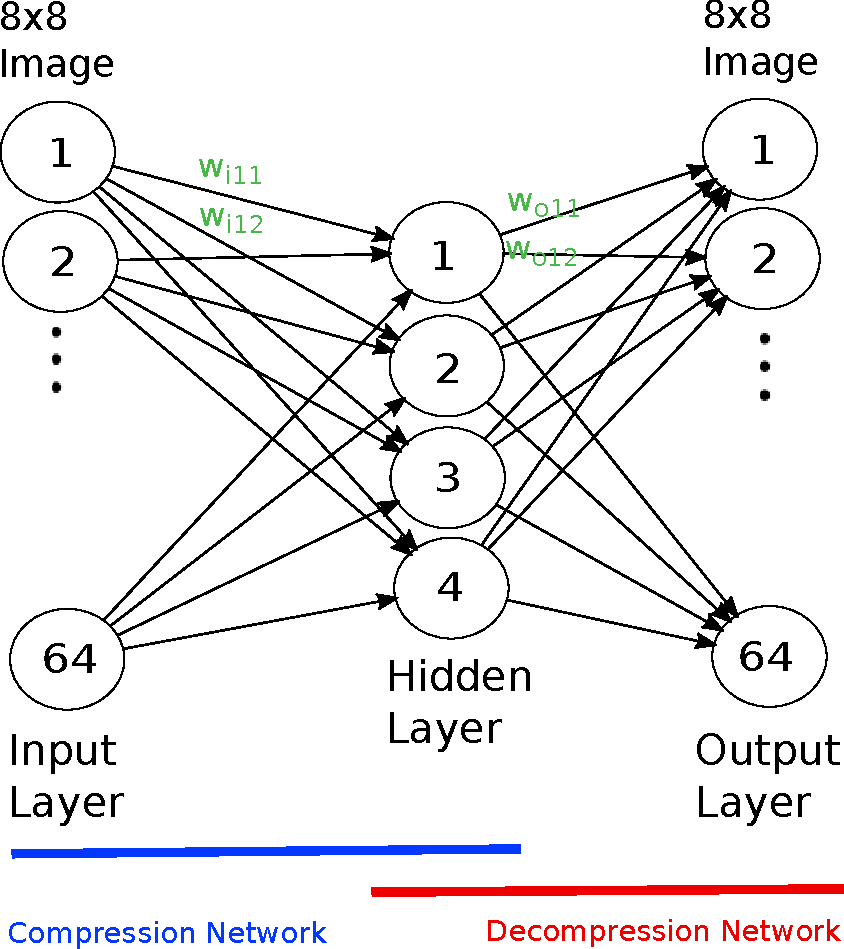
\includegraphics[width=\columnwidth]{images/nnStructure}
  \caption{Neural Network Structure for compression.}
  \label{fig:nnStructure}
\end{figure}

Figure~\ref{fig:nnStructure} shows the neural network structure we use for compression. There are three layers: input layer, hidden layer and output layer. The input layer and the hidden layer are fully interconnected as are the hidden layer and the output layer. The weights of the edges are detrermined by the training algorithm which is described in the next section. This kind of neural network is also called bottleneck-like neural network, because the hidden layer is a bottleneck.

\subsection{Neural Network Training Algorithm}
For the training 8 by 8 chunks of the image are chosen uniformly at random. The output of the bottleneck-like neural network has to be the same as the input and the weights are set accordingly. This process is iterated until the image is reconstructed faithfully.  
Different learning methods were tried like (....TODO) but it turned out that for the Levenberg-Marquardt method the results were best. 
\subsection{Singular Value Decomposition}
The singular value decomposition(SVD) is a matrix factorization. A m$\times$n matrix M can be written as a product of three matrices U, $\Sigma$ and V$^*$, where U is a unitary m$\times$m matrix, V$^*$ is the conjugate transpose of a n$\times$n unitary matrix V and $\Sigma$ is a m$\times$n diagonal matrix. The entries on the diagonal of $\Sigma$, which are non-negativ real numbers, are called the singular values of M. The columns of U are called left singular vectors and the rows of V$^*$ are called right singular vectors of M. \\
SVD can be used for image compression the following way. The singular values are sorted in descending order and then only the largest singular values and the corresponding right and left singular vectors are used to save the image.

\subsection{Quanitization}
\label{sec:quanitization}
\begin{figure}[tbp]
  \centering
  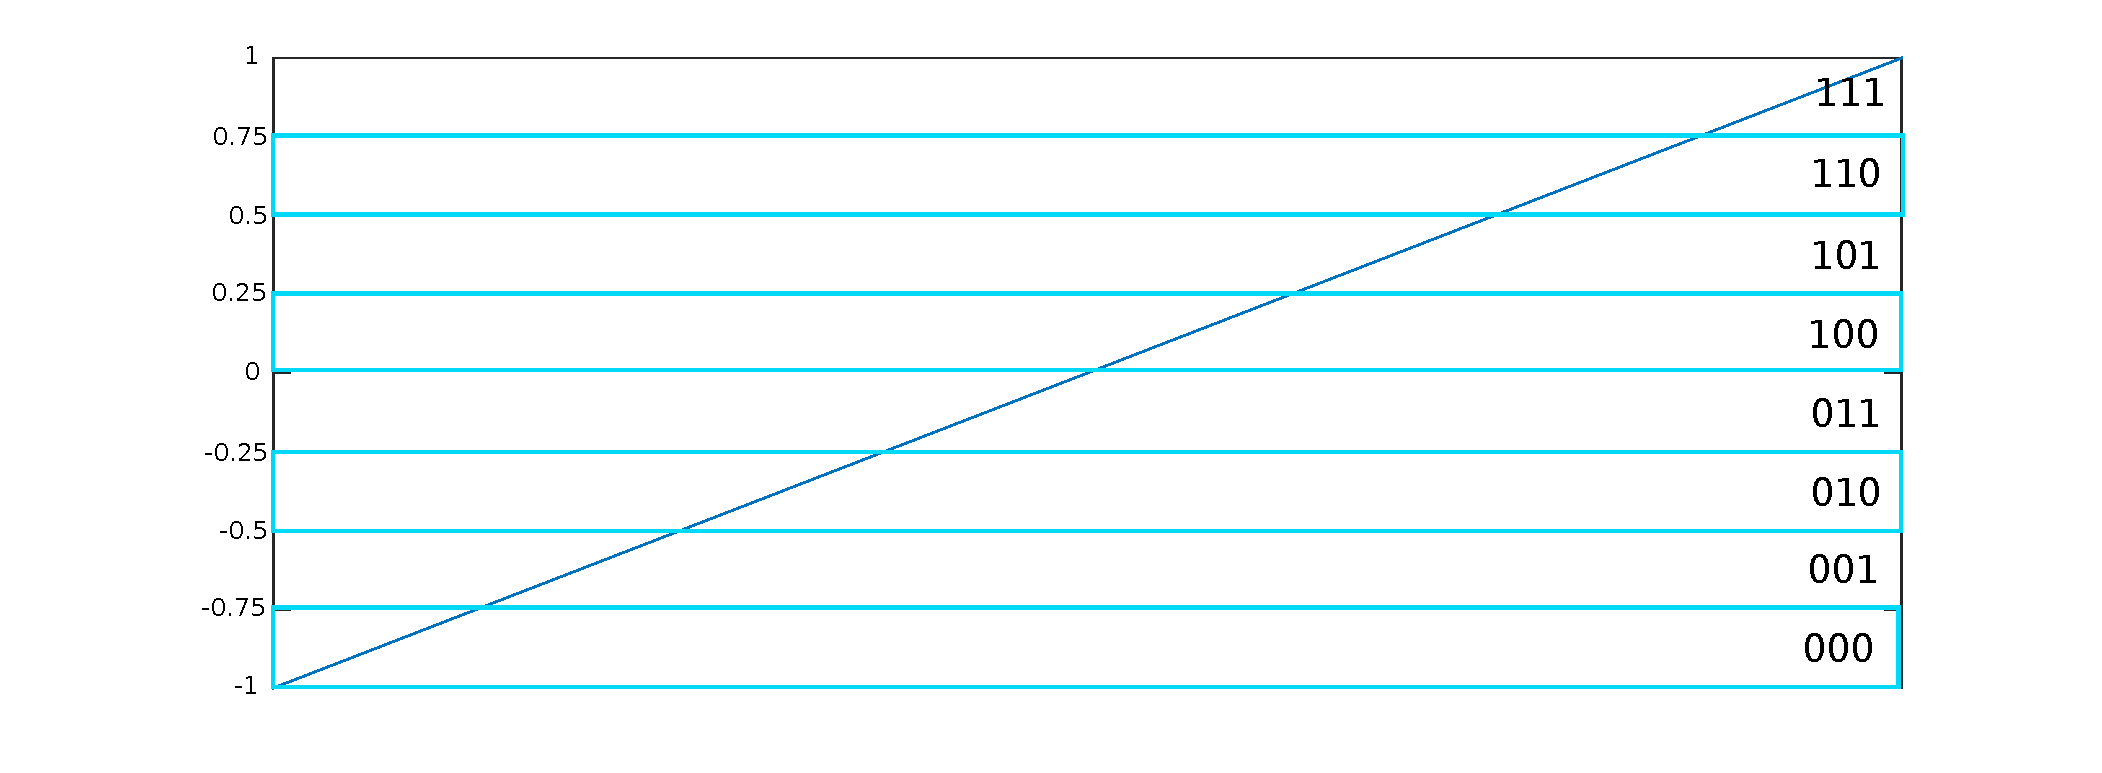
\includegraphics[width=\columnwidth]{images/bqQuantizer}
  \caption{Neural Network Structure for compression.}
  \label{fig:bpQuantizer}
\end{figure}

Quantization as shown in Figure~\ref{fig:bpQuantizer} is the process of mapping a large set of values to a smaller set of values. In Figure~\ref{fig:bpQuantizer} we construct 8 possible binary codes which can be represented with 3 bits. Each code represents an interval of the decimal values. For example, for the values between -1.0 and -0.75 we use the code 000. This way, we use 3 bits for a pixel that originally is represented by 8 bits. This compression method is lossy and the original image can not be reconstructed. 
